\begin{figure}
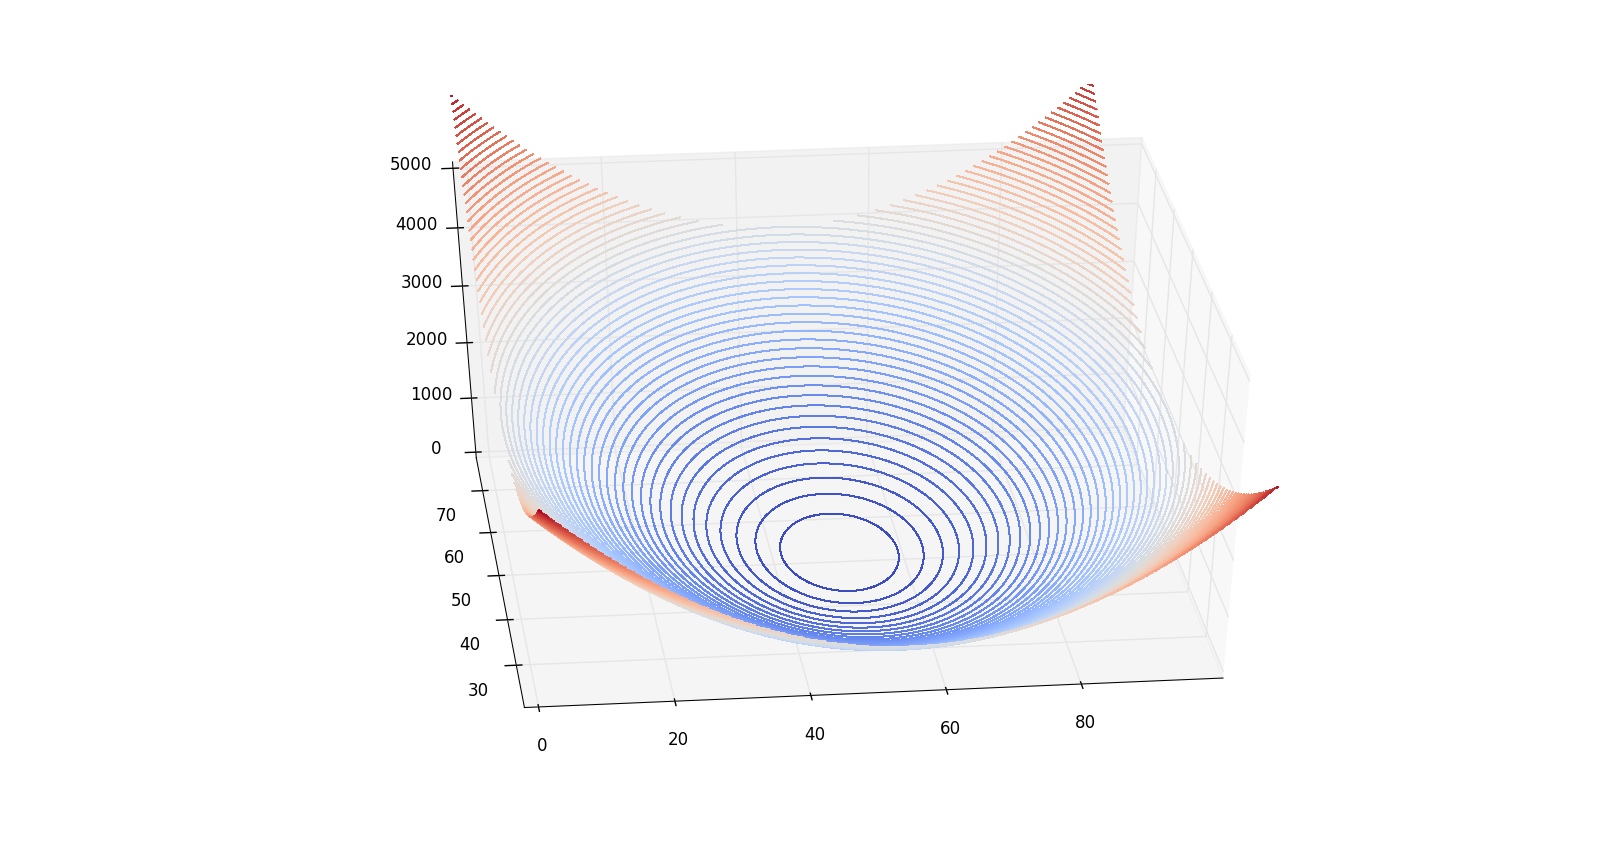
\includegraphics[height=.3\vsize]{fig/arriv1.png}
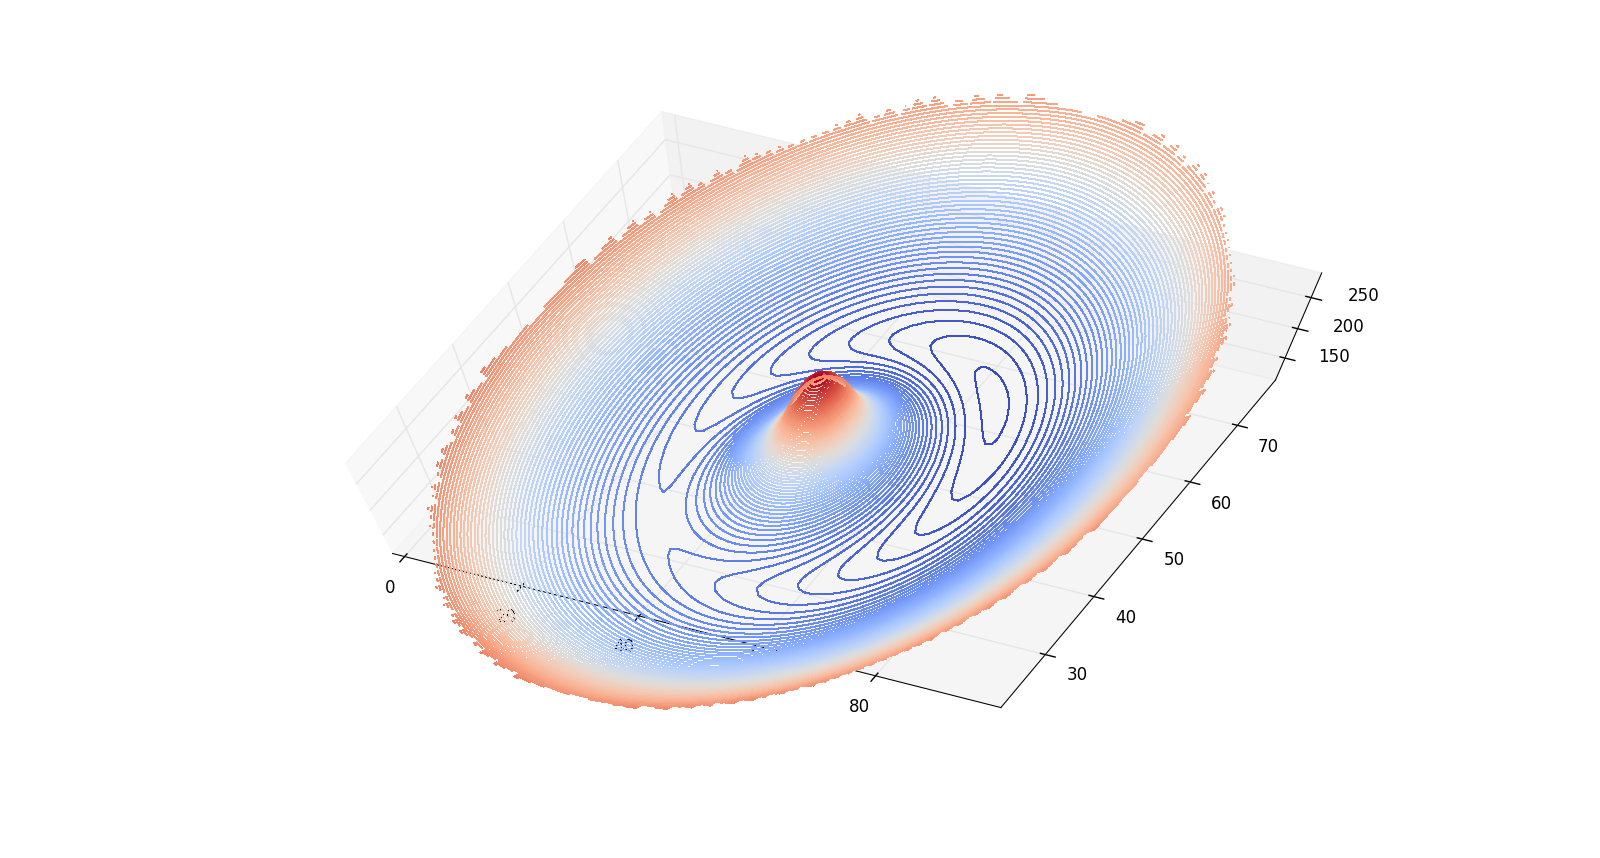
\includegraphics[height=.3\vsize]{fig/arriv2.png}
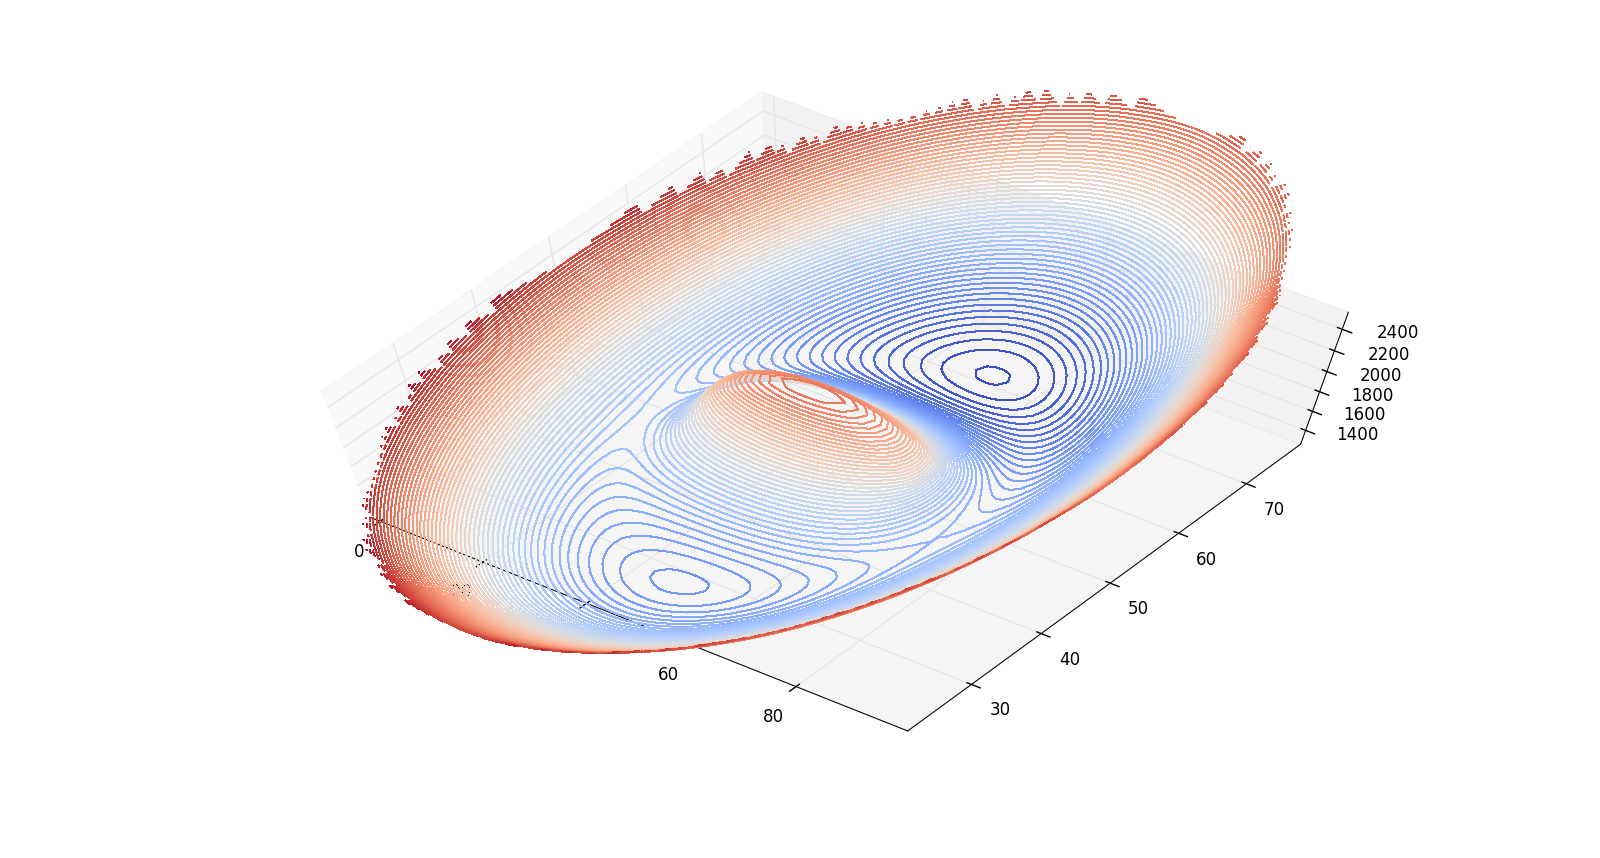
\includegraphics[height=.3\vsize]{fig/arriv3.png}
\caption{Arrival-time surfaces\label{fig:arriv}}
\end{figure}

\input{fig/sims/6941} % simple

\input{fig/sims/6975} % substructure ok

\input{fig/sims/6937} % substructure fail

\input{fig/sims/7022} % core quad

\input{fig/sims/6990} % long-axis quad

\input{fig/sims/6919} % incipient short-axis quad

\input{fig/sims/6915} % inclined quad

\input{fig/sims/6971} % wrong identification

\endinput

\input{fig/sims/6943}


\input{fig/sims/6916}


\input{fig/sims/7004}


\input{fig/sims/6995}







